\chapter{Úvod} \label{chap:introduction}
% \uv{Introduction section of your paper leads a reader from a well-known to the particular spot}

% Skeleton:
% \begin{itemize}
%     \item background
%     \item gap
%     \item proposed method
%     \item outline
% \end{itemize}

% motivace, zasazení do kontextu, o čem práce je, jaké jsou cíle práce, rozvržení práce (outline)


% background
Bezpilotní letadla se používají v~mnoha oblastech lidské činnosti mimo jiné díky nízkým nákladům na pořízení i provoz a vysoké manévrovatelnosti \cite{Hayat2016}. Široké uplatnění nachází v~oblastech jako je průzkum při mimořádných událostech a s~nimi související práce, monitorování prostředí \cite{Xin2022}, dopravní a bezpečnostní dohled, služba pátrání a záchrany, doprava zboží, zemědělství nebo při výstavbě a kontrole staveb \cite{Shakhatreh2019}. Součástí každé mise takového letadla je kromě samotné operace ve vzduchu také start a přistání. Řídicí systémy letadel obsahují funkce, které zajišťují jejich autonomii během startu i letu, ale kvůli složitosti manévru přistání a nedostatečné přesnosti obvyklých senzorů nedosahují potřebné spolehlivosti \cite{icuas}. Tato diplomová práce se zabývá využitím kamery a plošiny označené fiduciárním markerem pro automatizaci přistávání bezpilotního letadla se svislým přistáním v~simulovaném prostředí, vnějšími vlivy, které mohou přistávání ovlivnit a návrhem systému, který umožňuje efektivní testování různých metod přistávání. Jejím cílem je zhodnotit použitelnost různých simulátorů pro řešení úlohy přistávání a simulace vnějších vlivů, navrhnout simulační systém, s~jeho využitím vyzkoušet různé dostupné metody přistávání a vyhodnotit jejich vlastnosti z~různých hledisek ve vztahu k~simulovaným vnějším vlivům.

\section{Bezpilotní letadlo}
Bezpilotním letadlem se rozumí zařízení, které je schopné vyvozovat síly nesoucí ho v~atmosféře, které nejsou reakcemi vůči zemskému povrchu a je způsobilé létat bez pilota, tzn. je za letu řízené automatickým zařízením nebo dálkově ze země a označuje se také jako dron nebo zkratkou \acrshort{uav} z~anglického unmanned aerial vehicle. Obecně se může jednat o~letadla lehčí než vzduch (např. balony, vzducholodě) i těžší než vzduch (např. letadla s~nepohyblivými nosnými plochami, rotorová letadla). \cite{csn310001} Praktické využití přistávání na plošině se týká pouze letadel se svislou dráhou přistání a pro účely této práce budou uvažována pouze malá vícerotorová letadla nebo také multikoptéry. Experimenty (\cref{chap:eval}) byly provedeny s~letadlem o~4 rotorech.

\subsection{Komponenty malého vícerotorového letadla}
Vícerotorová letadla mají konstrukční, pohonné a řídicí součásti, které dohromady určují jeho letové vlastnosti jako jsou nejvyšší přípustná hmotnost nákladu, dynamické vlastnosti, dolet atp., podle nichž mohou být daná \acrshort{uav} vhodná jen pro určitou oblast aplikace, a dále palubní příslušenství, které se volí podle plánovaného využití. Základní schéma pohonných a řídicích součástí je na \refskl{fig:dronSoucasti}{obrázku}.

Hlavní konstrukční součástí je rám, ke kterému jsou připevněny ostatní komponenty. Obvykle má paprsčité uspořádání v~jehož středu se nachází převážně řídicí komponenty a jehož ramena na koncích nesou motory s~vrtulemi. Na různých místech rámu mohou být pomocí držáků a nosičů dále připevněny přídavné senzory závislé na aplikaci (barevné kamery, IR kamery a gimbaly, senzory vzdálenosti atd.), nožičky pro přistávání, antény pro rádiovou komunikaci s~pozemní stanicí nebo jinými letadly (např. při použití ve skupině více letadel) nebo ochranné rámy pro použití v~blízkosti překážek nebo v~interiéru. V~závislosti na počtu rotorů a jejich uspořádání se rozlišují různé konfigurace rámu, jejich příklady jsou na \refskl{fig:konfigurace}{obrázku}.
\begin{figure}
    \centering
    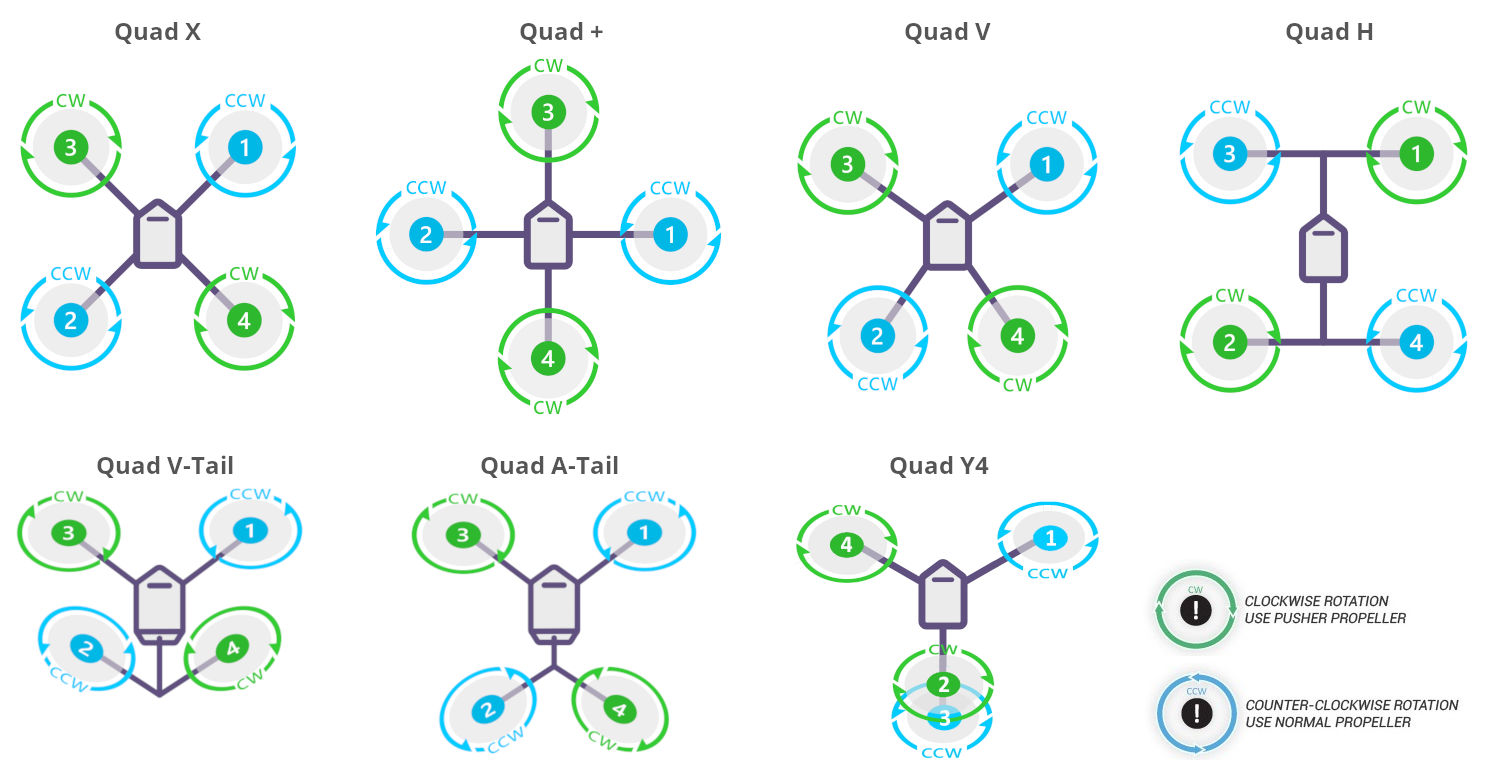
\includegraphics[width=0.9\textwidth]{img/intro/konfigurace.jpg}
    \caption[Uspořádání rotorů rámů u~čtyřrotorových letadel]{Příklady uspořádání rotorů a rámů u~čtyřrotorových letadel. Zeleně značené rotory se točí v~záporném směru, modré v~kladném. Převzato z~\cite{ardupilot} a upraveno.}
    \label{fig:konfigurace}
\end{figure}

Pohonné součásti jsou ty, které slouží k~zajištění vztlaku potřebného pro let a jsou ovládány řídicími součástmi. Letadla tohoto druhu jsou téměř výhradně elektrická napájená akumulátory. Každý z~rotorů je poháněn obvykle elektronicky komutovaným stejnosměrným motorem zapojeným do elektronického kontroléru rychlosti (\acrshort{esc}), jenž je ovládán řídicí jednotkou dronu a dodává motoru energii z~akumulátoru. Směr otáčení jednotlivých rotorů a jejich počet je často volen tak, aby bylo možné kompenzovat moment působící na letadlo otáčením vrtulí, na \refskl{fig:konfigurace}{obrázku} je toto vyobrazeno modrou a zelenou barvou rotorů. V~případě uspořádání s~lichým počtem rotorů je nutné použít jiný způsob kompenzace, např. pomocí umístění jednoho z~rotorů na pohyblivý kloub a tím řízení směru vytvářeného vztlaku.

Řídicí součásti zahrnují senzory, které poskytují informace o~poloze \acrshort{uav} v~prostředí a letovou řídicí jednotku, jež tyto vstupy zpracovává pomocí letového řídicího softwaru a na základě vstupů od pilota nebo požadavků autonomního řízení generuje řídicí zásahy pro motory nebo další aktuátory. Mezi senzory patří zejména \acrfull{imu}, přijímač \acrshort{gps} a nějaký senzor výšky (např. barometr), které dohromady slouží k~odhadu absolutní polohy v~prostoru a následnému řízení letadla dle dalších požadavků (pilota či programu).

\begin{figure}
    \centering
    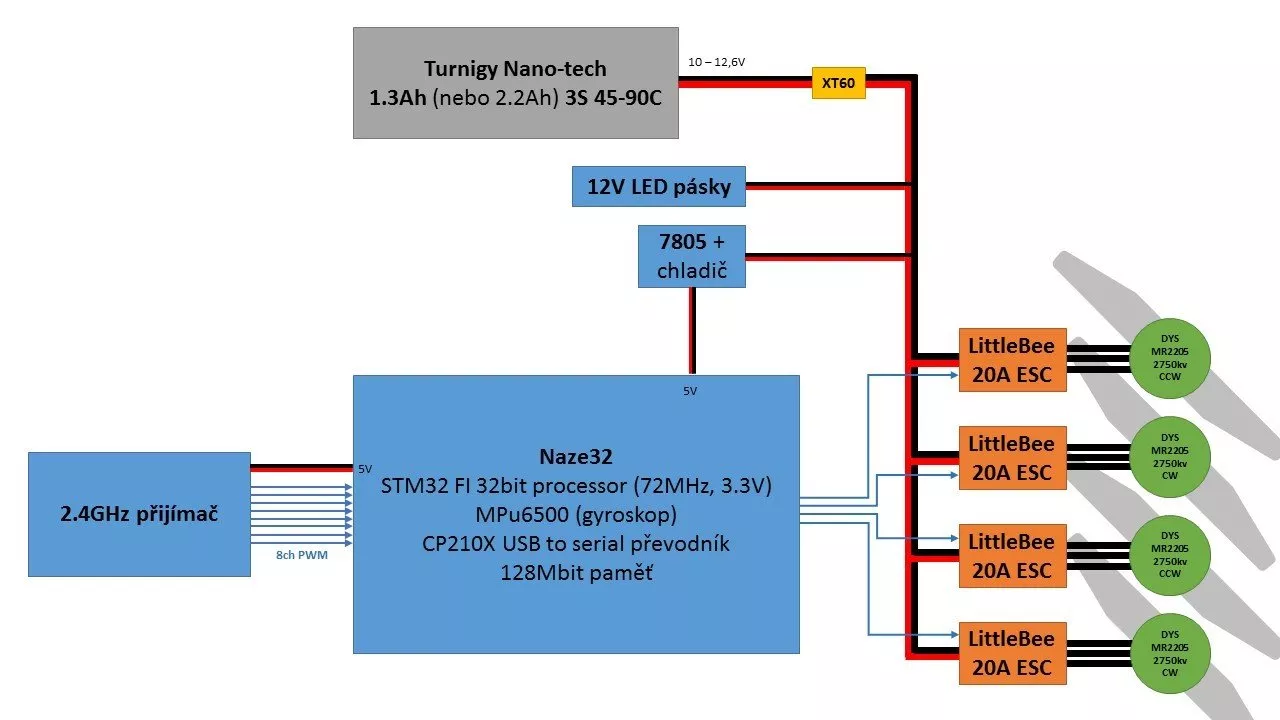
\includegraphics[width=0.9\textwidth]{img/intro/schema-kvadrokoptera.png}
    \caption[Schéma zapojení součástí letadla]{Blokové schéma zapojení základních řídicích a pohonných součástí kvadrokoptéry. \cite{dronSoucasti}}
    \label{fig:dronSoucasti}
\end{figure}

\section{Přistávání}
Konečnou fází letu je u~letadel včetně \acrshort{uav} přistávání, které je pro jejich plně autonomní využití potřeba automatizovat. Na základě odhadu polohy je možné pomocí běžných řídicích systémů \acrshort{uav} (např. těch uvedených v~\refskl{chap:sims}{kapitole}) automaticky přistát na zvoleném místě. Problém však tvoří nedostatečná přesnost lokalizace a tím snížená bezpečnost manévru.

Řešením nepřesnosti může být nějaké přídavné lokalizační zařízení (např. radar nebo systém real-time kinematic - \acrshort{rtk} \cite{rtk}, který umožňuje výrazně zpřesnit odhad polohy pomocí \acrshort{gps}). Taková zařízení ale vyžadují další nastavení na místě použití \acrshort{uav} a jejich hardware je obvykle nákladný.

Vhodnou alternativou může být plošina s~fiduciárním markerem, který bude detekovat kamera dronu a na základě jeho umístění a tvaru v~obrazu určí polohu plošiny, na kterou tak vhodně řízené letadlo bude moci dosednout.
definice, možnosti, navádění na cíl (opticky, proč ne jiné možnosti)
\section{Struktura práce}
Tato diplomová práce je rozdělena celkem do 11 kapitol (včetně této), přičemž \cref{chap:introduction,chap:task,chap:pad,chap:detection,chap:algs,chap:sims} jsou spíše teoretického rázu, uvadí čtenáře do problematiky, vymezují klíčové pojmy a popisují jejich příklady v~kontextu práce. Jsou představeny různé fiduciární markery, simulátory letu \acrshort{uav} a řídicí programy včetně zhodnocení jejich použitelnosti s~ohledem na cíle práce. Také jsou uvedeny různé metody přistávání, které se objevují v~literatuře, a pro další zkoumání v~praktické části jsou z~nich odvozeny 4 vlastní metody.

Praktická část (\cref{chap:system,chap:gui,chap:eval,chap:discussion}) se zabývá návrhem systému pro simulaci přistávání \acrshort{uav} (\cref{chap:system}), pomocí kterého je možné implementované metody uplatnit v~umělém světě a sledovat jejich vlastnosti, včetně grafického uživatelského rozhraní (\acrshort{gui}, \cref{chap:gui}), díky kterému může uživatel snadno spouštět simulaci za různých podmínek a zaznamenávat její výsledky. Zjištění jsou diskutována v~\cref*{chap:discussion}. kapitole a celou práci shrnuje závěr (\cref{chap:conclusion}), po němž jsou uvedeny veškeré informační zdroje, ze kterých bylo čerpáno při vypracování. Implementace navrženého systému a metod přistávání je dostupná na webu na adrese: \url{https://github.com/pernik36/dp-uav-landing}.